\documentclass[UKenglish, a4paper]{ifimaster}
\usepackage[latin1]{inputenc}
\usepackage[T1]{fontenc,url}
\urlstyle{sf}
\usepackage{babel,textcomp,csquotes,ifimasterforside,varioref,graphicx}
\usepackage[backend=biber,style=numeric-comp]{biblatex}
\usepackage{pifont}
\usepackage{booktabs}
\usepackage{verbatim}
\usepackage{listings}

\lstset{%
    captionpos=b,
    tabsize=2,
    breaklines=true
}

\newcommand{\cmark}{\ding{51}}
\newcommand{\xmark}{\ding{55}}
\newcommand{\ampers}{\&}
\newcommand{\demo}{VizPub}

\title{Visualizing and Evaluating the Performance of Overlay-Based Pub/Sub Systems}
\subtitle{}
\author{Nils Peder Korsveien}

\addbibresource{bibliography.bib}

\begin{document}
\ififorside{}
\frontmatter{}
\maketitle{}

\chapter*{Abstract}
\tableofcontents{}
\listoffigures{}
\listoftables{}
\chapter*{Aknowledgements}
\mainmatter{}

\chapter{Introduction}
\section{Thesis Outline}

\section{Motivation}

The publish/subscribe communication paradigm is receiving an increasing
amount of attention from the research community, as it provides a
loosely coupled and scalable interaction scheme suitable for large-scale
distributed systems~\cite{Eugster:2003}. It has also shown to be a useful
approach for several business applications such as financial data
dissemination~\cite{tibcorv} and application integration~\cite{goops}.
Topic-based pub/sub has also seen more novel applications such as
decentralised social networks. More specifically, the issue of
delivering notifications in such a network is a task especially suited
for this approach. This motivates further investigation into such
systems, comparing their performance and analysing their
characteristics and shortcomings.

\section{Problem Statement}


\chapter{Background}
%Provide background of
- pub/sub systems
- p2p
- overlay
- social networks
- metrics?
- visualizations
- gephi
- peernet
- briefly describe poldercast and scribe

\label{ch:background}
\section{The Peer-to-Peer Network Architecture}
In the peer-to-peer network architecture, every node in the network
contributes with its resources, including both storage space and
processing power.

%TODO read xl survey introduction for a good description

\section{The Publish-Subscribe Communication Paradigm}

Publish-Subscribe is a fully asynchronous, loosely coupled,
highly scalable, event-based messaging pattern. There are three main
system components in the pub/sub interaction scheme: the publishers, the
subscribers and the event service. The publishers publish events, and
the subscribers subscribe for events, while the event service handles
managing both subscriptions and publications, as well as routing events
to the subscribers. The basic architecture of a typical pub/sub system
is outlined in Figure~\ref{fig:pubsubarch}.

\begin{figure}
\centering
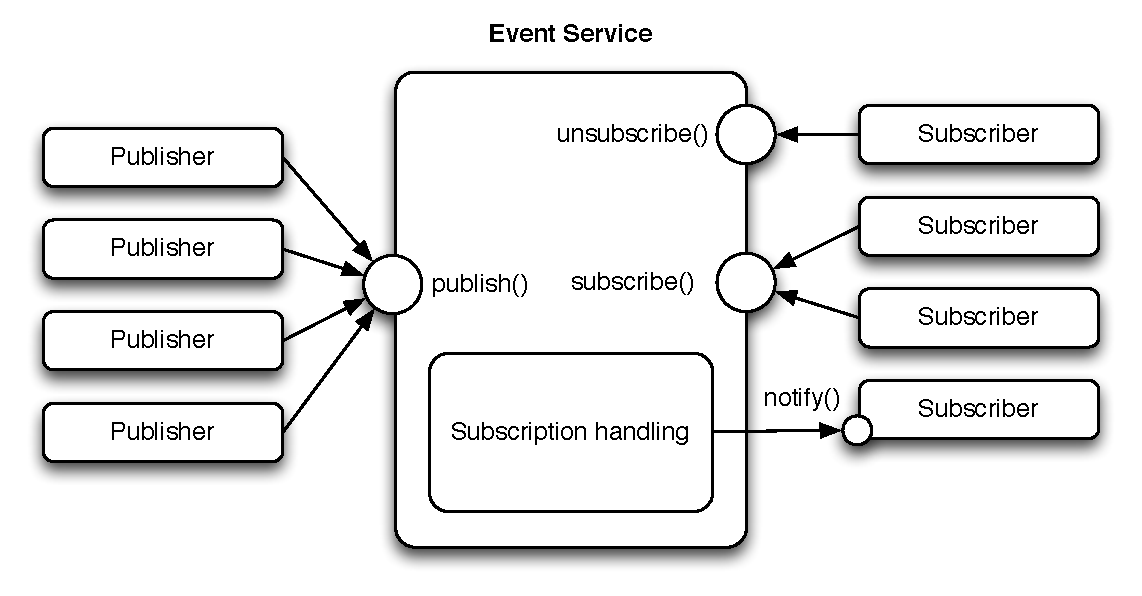
\includegraphics[width=\textwidth]{figures/pubsubarch}
\caption{The basic architecture of a pub/sub system.}
\label{fig:pubsubarch}
\end{figure}

The event service functions as an intermediary between publishers and
subscribers. It provides a level of indirection, as well as an service
interface. Publishers are able to generate new events through the
\texttt{publish} service call. It is now the responsibility of the event
service to determine which subscribers are interested in receiving this
event, and how to route the event to them. The subscribers register
their interest through a \texttt{subscribe} service call. The event
service will then store each subscribers interest in order to
disseminate events correctly. The publishers are then able to cancel
their subscriptions through a \texttt{unsubscribe} service call. No
information is forwarded from subscribers to publishers or from
publishers to subscribers.

The pub/sub paradigm provides a higher degree of decoupling than other
traditional approaches. In general there are three types of decoupling
pub/sub system provides us with:

\begin{description}
  \item[Space decoupling] The publishers and subscribers does not need to
    know about each other.
  \item[Time decoupling] Events are delivered regardless of whether or
    not publishers and subscribers are online at the same time.
  \item[Synchronization decoupling] Neither publishers nor subscribers
    are blocked when attempting to perform their operations.
\end{description}

While many other approaches can provide the first two forms of
decoupling, the main advantage of pub/sub is its fully asynchronous nature.
Approaches such as tuple spaces or message queues cannot completely
provide this synchronous decoupling, as messages are retrieved in a
synchronous manner. This property is key to the suitability for pub/sub
in large distributed system.~\cite{Eugster:2003}

\subsection{Message Filtering in Pub/Sub}

The subscription semantics of the pub/sub paradigm plays an important
role in the performance and flexibility of the system as event messages
are routed and managed based on topic or content. There are three
distinct types of subscription schemes:

\begin{description}
  \item[Topic-based] Events are split into topics, usually represented by
      a string.
  \item[Type-based] Filters events based on the structure of the data.
      Provides type safety at compile time.
  \item[Content-based] Events are filtered based on a global
      list of universal event attributes.
\end{description}

Content-based provides better expressiveness in terms of filtering out
the relevant events. However, this comes at the cost of higher overhead
with regards to handling subscriptions. The complex filtering algorithms
limit the scalability of such systems with regards to the number of
subscriptions. Type based is similar to content-based in the sense that
the public members of the types together form a description of the
content of the event. Although this ties the implementation of the
pub/sub system closer to the programming language, it still suffers from
the same drawbacks as content-based.

Topic-based offer less expressiveness than the other two subscription
schemes, but better performance if the set of possible event properties
is limited. Also, topic-based is more suited for dissemination and
multicasting, as topics can be thought of as groups, where subscribing
to topic T can be equivalent to joining the group for that topic. This
is a common approach taken by several proposed pub/sub
systems\cite{needs citation}.

Traditionally, reliable multicasting of data through deterministic
dissemination has been the common approach. However, more recent
implementations investigate the potentials of probabilistic protocols,
which are more suited to the nature of decentralized systems and P2P.
These protocols do not guarantee full reliability, but provides a high
quantifiable \emph{probability} that events are delivered to all
subscribers.

\section{Overlays}

\section{The Gephi Open Graph Viz Platform}

\begin{figure}
    \centering
    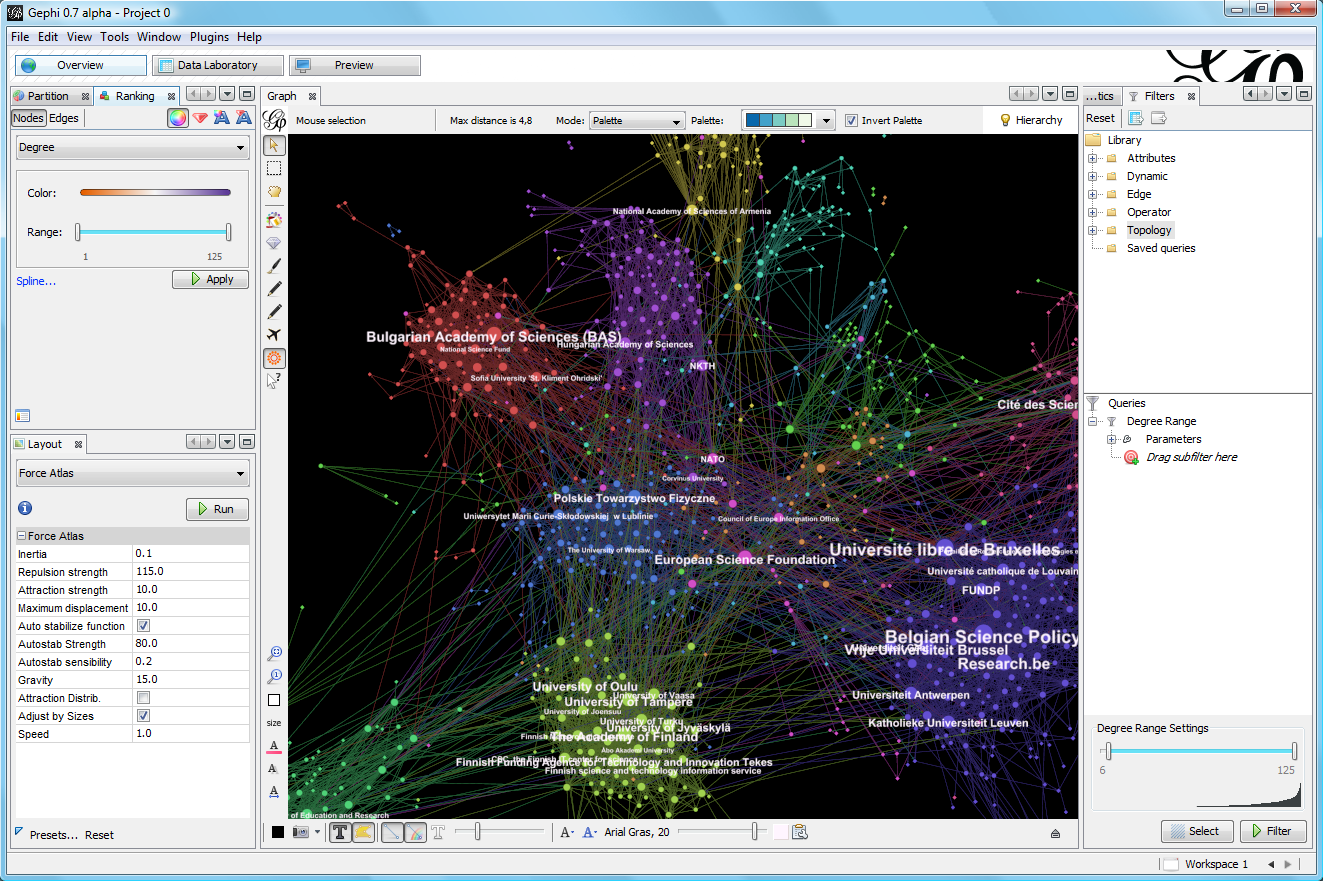
\includegraphics[width=\textwidth]{img/gephi1}
    \caption{The Gephi Tool supports
        visualization of graphs through coloring and sizing the visual
        graph
        representation. It also enables adding labels to nodes and
        edges. In
        this screenshot, Gephi is used to detect and visualize
    communities.}
\label{img:gephi1}
\end{figure}

Gephi~\cite{ICWSM09154} is an open source tool for exploring and
visualizing all kinds of networks, including dynamic and hierarchical
graphs. Described by the authors as ``photoshop for graphs'', Gephi
enables the user to interact with the graph structure, as well as
manipulate the colors and sizes of the visual graph representation in
order to display graph properties in an intuitive way. Gephi aims to
help researchers and data analysts in discovering patterns and revealing
hidden properties of the graph in question, as well as easily
discovering errors in the dataset. Gephi also provides a set of
statistical tools for measuring common metrics for Social Network
Analysis~(SNA) such as centrality, as well as metrics useful for general
graph topology analysis such as degree, path length and clustering
coefficient. Gephi is also useful in the emerging field of Dynamic
Network Analysis~(DNA)  as it supports temporal graphs, giving the user
the ability to filter the graph model according to a defined time
interval. It also support playback of the graph evolution, as well as
visualizing changes to graph data over time through size, color and text
labels which can be applied to both nodes and edges.

Gephi provides a rich GUI-experience where users may interact with the
graph representation, apply layout algorithms, filter the graph
representation, execute metrics, apply color and size based on graph
properties and animate the graph evolving over time through the timeline
component. The Gephi software architecture is highly modular and
supports extensions via plugins, some of which are available in a
official plugin marketplace found at~\cite{gephimarketplace}. New
metrics, filters or database support may be implemented through such
plugins by developers and published to the marketplace free of charge.

Gephi provides many tools and components which are useful in the context
of researching and analysing pub/sub overlays.

\subsection{Useful functionality in Gephi}

\begin{description}

\item[Node and Edge pencil tools] \hfill \\

    These two tools enable the user to create nodes and edges by
    clicking in the graph view. Edges can be undirected or directed,
    where direction is indicated with an arrow. These two tools combined
    enables building a graph by hand.

    Building such graphs can be useful in order to reason, analyse or
    learn network algorithms, such as event dissemination algorithms. In
    this case, the user can start with a single node which can act as
    the event source, and build the topology as the event disseminates,
    carefully following the particular algorithm in question when doing
    so. The user can also add attributes to the nodes and edges either
    through the node query tool or in the Data Laboratory component
    which also aids in visualising and understanding properties,
    drawbacks and advantages of such algorithms.

\item[Node Query Tool] \hfill \\

    With the node query tool the user is able to click on a node on the
    graph model, and a panel which will display a panel with information
    regarding the properties and attributes of this node. Properties include
    data describing the visual properties of the node such as size, position
    and color. Attributes include the Id and Label and Time Interval
    attributes and any additional user defined attributes. In our case, such
    user defined attributes would include Topics, Subscription Size and
    Gossips Sent/Received.

    Both the properties and attributes of the node are editable through this
    panel view. The user can select a property to change the visual
    representation of the node, or the attributes to change their value. The
    Time Interval attribute is interesting to edit in particular as it
    represents the points in time in which a node exists in the graph model.
    On example scenario is editing the Time Interval attribute for a certain
    nodes in order to see how it affects a particular metric as well as the
    overlay topology.

\item[Shortest Path Tool] \hfill \\

    With the Shortest Path Tool selected, the user may click on two nodes on
    the graph model, and if there is a shortest path between them, this path
    will be highlighted with a color. It might be useful to reason about the
    relationship between key nodes in the graph, or to compare shortest path
    between several pairs of nodes. (more use cases?)

\item[Heat Map Tool] \hfill \\

    The heat map tool enables the user to click on a node in the graph model
    and color its neighborhood based on the edge weight distance between
    them. More specifically, it sets the node color intensity lower for more
    distant nodes and stronger for nodes that are closer. Edge weight is a
    standard edge attribute that are by default set to 1. This means that in
    the default case, the visualization will represent the hop count
    distance from the particular node selected by the user. However, the
    edge weight can be edited by the user in order to represent other
    properties of a system. As an example, imagine setting the edge weight
    to represent network latency between two nodes. In this case, a
    neighboring node which is adjacent to the selected node would have a
    lower color intensity if the latency between them is higher than another
    neighboring node which is further away in terms of hop count.

\item[Timeline Component] \hfill \\

    The timeline component introduces an animation scheme for dynamic
    graphs. The user may choose playback parameters such as time
    interval size, step size and playback speed. The time interval will
    filter out a subgraph defined by the upper and lower bound of the
    interval. The evolution of the dynamic graph will then be animated
    by moving these bounds by the distance defined by the step
    parameter. The delay between each step is decided by the playback
    speed.

    The timeline enables the user to visually inspect the change in
    graph topology over time, as well as visualize and inspect node and
    edge attributes of the graph through both color, size and text
    labels which is able to change dynamically as part of the graph
    model animation. The timeline also enables jumping to a specific
    point in time and investigating the corresponding subgraph and its
    properties by changing the upper and lower bound of the Time
    Interval.

\item[Statistics Component] \hfill \\

    The metric component enables graph topology analysis by executing
    metrics on the graph. There are two types of metric algorithms in Gephi:
    static and dynamic. Static metrics are only able to execute on graph
    model representing a single point in time, while dynamic will traverse
    the time line by executing the metric iteratively across a set of time
    intervals. When executing a dynamic metric, the user is able to choose
    window size and time step. The window size is a time interval which will
    be moved by the step size defined by the user. Metrics are divided
    into \emph{static} and \emph{dynamic} metrics, where the former
    calculates a single value based on the currently defined time
    window, while the latter calculates a time series of values. When
    executing a dynamic metric, the user must define the time window
    size, and tick. The have the same functionality as step parameter
    when using the \emph{Timeline Component}. When the metric executes,
    the time window will iterate through the entire time range of the
    simulation, calculating a static metric at each step. When finished,
    a time series is plotted and displayed for the user.

    The Statistics component include several metrics which are relevant
    to pub/sub overlays. Useful static metrics include, but are not
    limited to:

    \begin{itemize}
        \item{Degree (In/Out/Avg./Max/Min/Distr.)}
        \item{Avg. Cluster Coefficient}
        \item{Centrality (Beetweeness/Closeness/Eccentricity)}
        \item{Average Path length}
        \item{Radius}
        \item{Network Diameter}
        \item{Number of Shortest Paths}
    \end{itemize}

    Of these, only degree and the clustering coefficient metrics have dynamic
    versions, where both calculates the average value over time. The
    average for dynamic metrics are calculated by dividing the sum of
    all node attribute values with the total number of nodes in both
    cases.

    %TODO: describe exactly what sort of averages/data are calculated by
    each metric

\item[Ranking Component] \hfill \\

    The ranking component is a key feature of Gephi which enables
    visualization based on node or edge attributes in form of color
    and size. When coloring nodes or edges, the ranking component
    will apply a gradient over the range of attribute values. The
    ranking component also include a Result list, where the user may
    sort nodes based on the specified attribute value, which is
    useful for quickly finding the nodes with maximum value and
    minimum value, which might help in identifying bottlenecks in
    the system or potential load balancing issues.

    The Ranking component also includes an Auto Apply feature, which
    supports vizualising attributes dynamically while playing back the
    graph via the Timeline Component.

\item[Layout Component] \hfill \\

    The Layout component enables the user to execute algorithms that
    calculates the position of the nodes. The user is able to adjust the
    parameters of these algorithms in order to manipulate the visual
    layout. The different algorithms emphasize different aspects of the
    topology. One example is the Force Atlas layout algortihm which
    simulates the effect of gravity on the nodes where linked nodes
    attract each other, and non-linked nodes are pushed apart. This
    particular algorithm is useful for visually detect clusters and
    communities. Another useful algorithm is the Circular Layout
    algorithm, where nodes are positioned in a circle ordered on a
    specific attributes selectable by the user. This is useful in order
    to visualize node rankings on particular attributes.

\item[Filter Component] \hfill \\

    Filter may be applied to the graph in order to strip away nodes or
    edges on the basis of their attributes which also includes any
    calculated metrics. Filters may strip away based on a value range if
    the attribute type is a number, or a regex match if the attribute is
    a string. Filters can be combined through special operator filters
    representing set operations such as union and intersect.

    Filters are an essential mechanism in order to analyze subgraphs.
    One use example is the case of calculating topic diameters in pub/sub systems,
    where a subgraph can be filtered on a topic attribute. This
    allows executing the diameter metric on the resulting subgraph
    on the selected topic.

\item[Data Laboratory Component] \hfill \\

    The Data laboratory component enables the user to work with the node
    and edge attributes of the graph. This component provides the user
    with separate table views of node and edge attributes. Each row in
    these table represent a node or edge, and columns may be added or
    removed by the user. The Data Laboratory also provides functionality
    for manipulating columns such as merging two columns or creating new
    columns based on data from the existing columns. Attribute data
    in columns that are static (i.e.\ has no lower or upper time
    interval bound associated with them) can be converted to dynamic
    through this component. Also, resizing or coloring all edges or
    nodes is possible through the laboratory by selecting all rows
    and right-clicking.

    The laboratory also enables the user to export the data to file
    for further statistical analysis.
\end{description}


We consider tools such as Gephi to be a valuable addition to the field
of P2P protocol research. Visual Exploration of a dynamic network graph
is a useful approach to evaluating these protocols, as some properties
of the system are more easily spotted visually. For example, during our
implementation work, it was trivial to visually confirm that some edges
were missing from the graph, leading to the discovery of a critical bug
in the implementation code which would otherwise be difficult to spot.
It is also worth to note that the different actors involved in the Gephi
project has formed a legal entity in the form of The Gephi
Consortium~\cite{gephi-consortium} in order to assure future development
of this tool. This provides us with a certain degree of assurance that
this project is something well worth investing in, as the risk of it
being discontinued seems unlikely at this point in time.

\section{The Gephi Toolkit}

In addition to the GUI-client, the authors of Gephi also provide an API
through the Gephi Toolkit project. The toolkit packages essential
modules from the GUI-client into a standard Java library which can
be used by any stand-alone Java project by including it as a dependency.
We take advantage of this toolkit in our implementation work, where it
is mainly used to handle and store reports collected from PeerNet
simulations.

\section{The GEXF File format}

The GEXF (Graph Exchange XML Format) file format~\cite{gexf} is an
effort by the Gephi Consortium to define a standard language describing
complex network structures. Being developed by the same group of people,
the Gephi Tool is naturally fully compatible with this format, and is
able to both import and export GEXF files. This is also the case with
the Gephi Toolkit, as the module for handling such imports and exports
are included in this toolkit as well.

The GEXF file format is able to describe a graph through its nodes and
edges, as well as any data and dynamics associated with the graph. More
specifically, the file format is able to describe node, edges and their
associated attributes. Listing~\ref{lst:gexf-basic} provides an example
of a minimal static GEXF file, describing nodes, edges and attributes of
a graph.

\begin{figure}
\lstinputlisting[language=XML, label=lst:gexf-basic, frame=single]{listings/basic.gexf}
\caption{A GEXF description of a minimal static graph}
\end{figure}

\subsection{Dynamics}

One of the major advantages of this file format is its support for
dynamic functionalities.  Both nodes, edges and attributes may have a
defined time interval where they exist. These lifetime intervals are
described as ``spells'' if applied to nodes and edges, and as ``start''
and ``end'' XML-attributes if applied to node or edge attributes. The
GEXF file in Listing~\ref{lst:gexf-dynamics} shows an example of a
dynamic graph where spells are used in order to determine the lifetime
of the nodes.  The start and end times are by default encoded as
doubles, however, dates are also supported, as seen in this example.

The
support for dynamic graphs makes this file format an interesting option
for storing simulation data, and in our implementation work we use this
format extensively as part of our research effort.

\begin{figure}
\lstinputlisting[language=XML, caption={}, label=lst:gexf-dynamics,
frame=single] {listings/dynamics.gexf}
\caption{Example of  dynamic GEXF file using spells}
\end{figure}

\section{The PeerNet Simulator}

\subsection{Event Engine}

\subsection{Protocols}

\subsection{Observers}



\chapter{Design Challenges in Topic-Based Pub/Sub}
% Provide a mini survey of existing pub/sub system. Might have to go
% through some rewrites.
\label{ch:design-challenges}
Designing decentralized topic-based pub/sub systems is a big research
challenge due to a number of desired system properties which are in
conflict with eachother. For example, making the
overlay robust is difficult without introducing too many redundant edges
in the network graph.  Many approaches to topic-based pub/sub have been
proposed the last
decade~\cites{Baehni:2004}{Castro:2002}{Chockler:2007}{Rahimian:2011}{Girdzijauskas:2010}{Matos:2010}{Wong:2008}{Zhuang:2001}.
And each have made trade-offs in an attempt to balance the system
properties against each other. In this chapter, we extend the
mini-survey found in~\cite{Setty:2012}, were we include a number of
additional protocols. Also, we will go more into detail regarding the
design challenges found in topic-based pub/sub system by illustrating
the charachteristics of these systems, as well as their shortcomings.

\section{Desired System Properties}

In order to provide correct and efficient delivery of notifications in a
decentralized OSN using topic-based pub/sub, a high number of system
properties are deemed desirable~\cite{Setty:2012}. More specifically,
these challenges include:

\begin{description}

    \item[Correct delivery]\hfill\\
        All notifications should be delivered to the
        correct recipient. Both false positives and false negatives should be
        avoided.

    \item[High hit-ratio during churn]\hfill\\
        Notifications are delivered to a very high
        percentage of subscribers in the presence of churn. In the
        absence of churn, notifications should be delivered to all
        subscribers. This is similar to correct delivery except for
        not taking false positives into account.

    \item[Fast recovery]\hfill\\
        The overlay should quickly recover from a
        period of churn. Nodes should be able to both leave and join the
        network gracefully, and nodes who are dead should be properly
        handled by the system.

    \item[Low average node degree]\hfill\\
        The overlay nodes should have a low
        node degree as possible to achieve scalability with regards to number of
        topics. The degree distribution should be as even as possible,
        in order to achieve load balancing.

    \item[Topic connectivity]\hfill\\
        The routing of an event only includes the
        subscribers who registered their interest for the topic. This is
        also known as \emph{relay-free routing}.

    \item[Scalability]\hfill\\
        The system should scale in terms of number of
        topics, number of nodes, number of topics a node is interested in and
        number of nodes interested in a topic.

    \item[Efficient dissemination]\hfill\\
        Event dissemination should have a low
        delay with little duplicate delivery, and the load of routing messages
        should be distributed fairly.

    \item[Low overlay maintenance cost]\hfill\\
        Managing the overlay topology
        should be as inexpensive as possible. Maintenance might include mending
        dissemination structures such as multicast trees when nodes fail, but
        also how to include joining nodes in the structure and allowing nodes to
        leave gracefully.

\end{description}

Designing a system with all of these properties
presents a challenge, as several of the desired characteristics are
fundamentally at odds with each other. Maintaining a low node degree
makes it difficult to maintain \emph{topic connectivity}, while
avoiding duplicate message delivery conflicts with being robust in the
presence of churn. There is also a trade-off in robustness and
reliability depending on the approach taken to disseminating messages.
Specialized overlays that build dissemination structures such as
multicast trees provide fast and reliable message delivery with no
duplication of messages. However, they are fragile and susceptible to
churn. Epidemic dissemination on the other hand is more robust, but does
not provide full reliability as it lacks deterministic delivery
guarantees.

There is also a trade-off between the navigability of the overlay and
the message overhead. Stanley Milgram famously demonstrated the
\emph{small-world phenomena} in~\cite{milgram1967small} where he showed
that any two participants in a network was likely to be connected
through a low number of intermediaries. Taking this phenomena into
consideration has proved to be a useful approach when constructing
decentralised overlays, as they provide a highly navigable network due
to the small average shortest path length. A popular approach is to
create one or more long jump links between nodes to provide better
routing capabilities. More specifically, these links are usually created
by utilizing a distance function in the name space, where the
probability of creating a link increases with the distance between them.
The subscription interest of such nodes are usually not taken into
consideration when creating such links. Consequently, the message
overhead in the system is increased as more relays are introduced in the
overlay.

Many existing systems suffer from shortcomings that originate from wanting
to include a high number of desired properties described above. This
motivates further research into these systems and how they compare in
terms of promoting these desirable properties.

\section{Handling Trade-offs}

Designers of existing approaches have been facing the challenges of
handling the trade-offs discussed in the previous section. One of these
challenges is building both a reliable and robust overlay. A naive
approach to this problem would be to create a separate overlay for each
topic as in TERA~\cite{Baldoni:2007}. However, this approach suffers from
poor scalability as the number of nodes and topics increase. Another
approach would be to structure the overlay by creating a spanning tree
per topic as seen in Scribe~\cite{Castro:2002}, Bayeux~\cite{Zhuang:2001}
and Magnet~\cite{Girdzijauskas:2010}. However, these structures are
conceptually fragile in the presence of churn, requiring mechanisms for
mending the structure when nodes fail. This increases the overhead of overlay
maintenance.  Also, the root node of the spanning tree represents a
single point of failure as well as a bottleneck in the system. This is
especially true for popular topics where all events must travel through
the root node. In Scribe, the root node is used as a \emph{rendezvous}
point for topics by using the routing capabilities of the underlying
Pastry DHT~\cite{Rowstron:2001}. Such dedicated nodes represent a
single point of failure in addition to being detrimental to load
balancing and scalability.

Minimizing the average node degree while simultaneously achieving a
\emph{topic-connected overlay} (TCO) is another difficult trade-off to
consider. Topic-connectivity is achieved when no other than the
nodes who registered their interest in a topic takes part in routing
events for that topic. The desired goal with regards to
topic-connectivity is not only to avoid routing events through
uninterested nodes, but also to minimize the node degree by reusing
links for several topics. This approach achieves better scalability with
regards to the number of topics in the system.  Also, it decreases the
message overhead incurred by both event dissemination and overlay
maintenance mechanisms such as heartbeat messages. In addition to this,
keeping an overlay topic-connected simplifies the message routing
mechanism as no designated relay or gateway node needs to be implemented
in the protocol such as in Scribe and Vitis.

ElastO~\cite{Chen:2013} propose an interesting approach to overlay
construction, where the goal is to construct a TCO while maintaining a low
node degree. The construction of the overlay is performed by a
centralized component which requires global knowledge, while the
maintenance of the overlay is performed in a distributed manner in
response to churn events. By using a centralized algorithm for overlay
construction, ElastO is able to provide a more optimal TCO than decentralized
solutions, while still maintaining the high performance of a
decentralized repair mechanism to handle node departure or arrival.

With regards to the reuse of links for several topics, an observed
correlation~\cite{Liu:2005} between subscription sets in practical
workloads is useful to consider when constructing overlays. This
observation is exploited in Poldercast in order to decrease the number of
links to maintain. Also, it is used as a basis for overlay construction
in both StaN~\cite{Matos:2010} and SpiderCast~\cite{Chockler:2007}.
However, these two protocols only provide a probabilistic guarantee that
the resulting overlay will be fully topic-connected. In contrast,
PolderCast claim deterministic guarantees of providing a TCO. However,
this relies on two factors: (1) that there is no churn in the system,
and (2) that the underlying Cyclon~\cite{Voulgaris:2005} protocol, which
is used for peer sampling in PolderCast, can guarantee a connected
overlay.  Consequently, the deterministic guarantees of PolderCast could
be questioned.\ daMulticast~\cite{Baehni:2004} on the other hand provide
a deterministic guarantee of topic-connectivity through quite a
different approach of overlay construction. More specifically,
daMulticast constructs a topic hierarchy, where events are disseminated
through gossiping each level of this hierarchy in a bottom-up approach.

As mentioned in section 2, several protocols attempts to create an overlay that
exhibits \emph{small-world properties}. In Vitis, the subcluster
together with the relay paths form an overlay similar to a small-world
networks, which decreases the routing delay, but includes
uninterested gateway and relay nodes. In Magnet, small-world properties
are provided by the underlying Oscar DHT~\cite{girdzijauskas2007oscar}
which cluster similar nodes together.

\subsection{Overlay construction}

There are several different approaches to overlay construction.
Structured approaches such as dissemination trees have already been
mentioned, but there are also unstructured approaches. In Quasar
\cite{Wong:2008}, a novel approach to event dissemination using random
walks removes the need for a structured overlay.  There are also hybrid
approaches to structuring overlays such as in ElastO~\cite{Chen:2013}
and Vitis~\cite{Rahimian:2011}. In ElastO, the bootstrapping of the
graph is performed by a centralized entity, while in Vitis nodes with
similar interests are clustered together. A topic in Vitis might consist
of several subclusters which are connected to each other through relay
paths. This creates an overlay that is similar to dissemination trees,
but where single nodes have been replaced with clusters of nodes.
However, the drawbacks are still similar to the ones found in systems
relying on multicast trees, as it relies on designated gateway nodes
within subclusters communicating with rendezvous nodes along the relay
path. In Poldercast~\cite{Setty:2012}, a structured ring per topic is
used in combination with a form of epidemic dissemination that resembles
gossiping. Publishers are themselves part of the ring of the topic they
publish, and the structures attempt to combined into themselves into a
single overlay through random links. Such an hybrid approach is an
attempt at balancing the reliability of a structured overlay with the
robustness of epidemic dissemination. When it comes to node degree
however, Poldercast might introduce hotspots in the system as the
distribution of random links might be skewed.

In Magnet, the aforementioned subscription correlation is used to build
dissemination trees such as the ones seen in Scribe and Bayeux. As
mentioned these structures are not ideal in dynamic systems as they
require maintenance. However, tree structures do have an advantage when
it comes communication overhead, as they in theory avoid any duplicate
messages. In practice however, duplicate messages might occur if a node
that is part of a tree is part of an underlying routing path to the root
node. For example, in Scribe, notifications are routed to the root node
of a topic tree using an underlying DHT. If a child node belonging to
this tree is part of the routing path, it will receive the same message
twice. Once while routing to the root, and once again from its parent
after the publication message has reached the root node. However, the
number of duplicates should still be lower than what is seen in systems
relying on epidemic dissemination schemes, such as daMulticast and
PolderCast. In such systems, the number of duplicate messages are indeed
higher, however, the increased number of control messages also has the
benefit of making these systems more resilient to churn. Furthermore,
there is usually an adjustable \emph{fanout parameter} in such systems
which can be manipulated in order to control the number of messages that
are forwarded by a node. Thus, there is some control over the amount of
communication overhead in these systems. Both PolderCast and daMulticast
include such a fanout parameter. Also, it bears mentioning that
structured overlays include communication overhead in the form of
structure maintenance and structure mending in the case of both node
failure as well as nodes leaving and joining the network. Control
messages such as heartbeats are commonplace in such protocols e.g.\ in
Scribe where the each non-leaf node in the multicast tree periodically
sends heartbeats to its children. This increases bandwidth consumption
and adds a higher communication overhead compared to unstructured
overlays where such maintenance usually is not required.

Node degree is another important issue to consider when designing
overlays. A low average node degree increases scalability as topics and
number of nodes in the system increases. In protocols who rely on an
underlying DHT, node degree is usually either constant or a logarithmic
function of the total number of nodes in the graph. Such is the case in
Bayeux which relies on the Tapestry DHT~\cite{tapestry}, or Scribe which
relies on the Pastry DTH~\cite{Rowstron:2001}. Other implementations
might have a constant node degree, which is the case in Vitis which
might result in the separation of a topic into subclusters. Some extreme
examples include TERA~\cite{Baldoni:2007} and
daMulticast~\cite{voulgaris:2007} which
has a node degree that grows in the order of the number of topics the
node has subscribed to.  In the worst case scenario, this is also the
case in PolderCast, as maintaining a low node degree depends on the
degree of correlation in the subscription sets.  Indeed, when using
workloads from Facebook, the node degree in PolderCast grows almost
linearly with subscription size, as shown in \cite{Setty:2012}. This
suggests a scalability issue in a scenario where the subscription
correlation is weak.

%{../tables/comp-overlay} <- vim gf
\begin{table}
\centering
\resizebox{\columnwidth}{!}{%
\begin{tabular}{ccccccc}
    \toprule
    Protocol                         & Overlay      & Structures? & TCO?\    & Central nodes* & sub.\ corr.? & Node degree \\
    \midrule
    Scribe~\cite{Castro:2002}        & Structured   & Trees       & \xmark{} & RV             & \xmark{}     & $O(\log|\mathcal{V}|)$ \\
    Magnet~\cite{Girdzijauskas:2010} & Structured   & Trees       & \xmark{} & Relays         & \cmark{}     & $O(1)$\\
    Bayeux~\cite{Zhuang:2001}        & Structured   & Trees       & \xmark{} & RV             & \xmark{}     & $O(\log|\mathcal{V}|)$\\
    Vitis~\cite{Rahimian:2011}       & Hybrid       & Trees       & \xmark{} & RV\ampers{}GW  & \xmark{}     & $O(1)$\\
    StaN~\cite{Matos:2010}           & Unstructured & None        & prob.    & None           & \cmark{}     & $O({|\mathcal{T}_v}|)$\\
    SpiderCast~\cite{Chockler:2007}  & Unstructured & None        & prob.    & WB             & \cmark{}     & $O(K\cdot(|\mathcal{T}_v|))$\\
    daMulticast~\cite{Baehni:2004}   & Unstructured & None        & det.     & None           & \xmark{}     & $\Theta({|\mathcal{T}_v}|)$\\
    Quasar~\cite{Wong:2008}          & Unstructured & None        & \xmark{} & None           & \xmark{}     & Unknown\\
    PolderCast~\cite{Setty:2012}     & Hybrid       & Rings       & det.     & None           & \cmark{}     & $O({|\mathcal{T}_v}|)$\\
    ElastO~\cite{Chen:2013}          & Structured   & Ring        & det.     & None           & \xmark{}     & $O({\rho \log |\mathcal{V}}| |\mathcal{T}|)$\\
    \bottomrule
    \multicolumn{5}{l}{*RV:\ Rendezvous GW:\ Gateway WB:\ Weak bridge}\\
\end{tabular}
}%
\caption{Comparison of the different protocols and their overlay properties}
\label{table:comp-overlay}
\end{table}


Table~\ref{table:comp-overlay} provides an overview over several
different state-of-the-art protocols, comparing their different system
properties such as topic connectivity and whether or not it takes
advantage of subscription correlation.  Note that
PolderCast has received the benefit of doubt in this table, and have
been marked as providing a deterministic guarantee of
topic-connectivity. Magnet has a different approach to the spanning tree
structures, where messages are disseminated bottom-up. This means that
the root node is not a rendezvous node according to  the traditional
definition~\cite{baldoni2005distributed}, but it is still conceptually
a single point of failure as it is responsible for propagating messages
back down the tree when it receives a message. In SpiderCast, there is a possibility
of the overlay forming into a pattern of highly connected clusters
inter-connected through a small number of links which we refer to as
\emph{weak bridges}. The node degree in SpiderCast also relies on the
\emph{K-coverage} parameter of the system, where, for each topic, a node
attempts to connect to $K$ neighbours who share the same interest.
Protocols who rely on a underlying DHT typically have a node degree
which grows logarithmically with the number of nodes in the system. The
exception is Magnet which leverages a DHT providing small-world
properties~\cite{girdzijauskas2007oscar}, creating a fixed node degree
that is independent of both subscription size and number of topics
\cite{Zhuang:2001}.  Note that the node degree in Quasar is omitted from
the table, as it is dependent on the implementation of the bloom filters
used to represent the neighbours. In ElastO, $\rho$ is a system parameter
which balances between average and maximum node degrees when choosing
new edges to recover from churn.

% Note that even though ElastO has a
% higher node degree than the centralized solutions, it provides a more
% optimal TCO.\

\section{Event dissemination}

In terms of event dissemination, it should be mentioned that some of
the systems described earlier do not concern themselves with this aspect, and
focus only on the construction and maintenance of the overlay
itself. More specifically, this includes SpiderCast, StaN and ElastO. Thus, any
discussion regarding dissemination technique or routing performance
will be irrelevant for these systems. For other systems however, a
comparison of techniques is in order.

As mentioned, the dissemination in systems relying on multicast trees
removes much of the message duplication and usually offers on average
dissemination of events in logarithmic time as is the case in Scribe,
Magnet and Bayeux. In Vitis, event dissemination is performed by
flooding inside the subcluster, while simultaneously forwarding the
event to other subclusters if needed. As mentioned, gossiping is the
main approach in both daMulticast and PolderCast.  Gossiping usually
implies an exponential dissemination speed, however, there might be
other implementation specific factors in play which inhibits this
property of gossiping. As an example, in PolderCast, skewed random link
distribution might be detrimental to the speed of the gossiping
protocol. The authors of Quasar~\cite{Wong:2008} propose quite a different approach
to event dissemination, as routing is performed by having nodes install
routing vectors in nearby overlay neighbours. Messages are disseminated
through random walks, which are directed towards the subscribers when
passing through a node with the relevant routing information. This
approach is likely to be highly robust against churn. However, as
observed in~\cite{Wong:2008} the hit ratio stagnates at 97\% in a
static system. This is due to a phenomenon where some group members
might be obscured by other members who absorb messages
from all directions. The authors suggest a solution by having node
periodically pull information from other nodes, but this introduces more
overhead in terms of network traffic and data processing.

%{../tables/comp-dissemination} <- vim gf
\begin{table}
\centering
\resizebox{\columnwidth}{!}{%
\begin{tabular}{ccccc}

\toprule
Protocol                         & High hit-ratio during churn & 100\% hit-ratio in absence of churn & Message Delay              & Avg.  Duplication Factor \\
\midrule
Scribe~\cite{Castro:2002}        & \xmark{}                    & \cmark{}                            & $O(\log|\mathcal{V}|)$     & None\\
Magnet~\cite{Girdzijauskas:2010} & Unknown                     & Unknown                             & $O(\log|\mathcal{V}|)$     & None\\
Bayeux~\cite{Zhuang:2001}        & Unknown                     & Unknown                             & $O(\log|\mathcal{V}|)$     & None\\
Vitis~\cite{Rahimian:2011}       & \cmark{}                    & \cmark{}                            & $O(\log^2|\mathcal{V}|/k)$ & Scoped flooding\\
daMulticast~\cite{Baehni:2004}   & \cmark{}                    & \xmark{}                            & $O(\log|\mathcal{V}|)$     & Gossiping\\
Quasar~\cite{Wong:2008}          & \cmark{}                    & \xmark{}                            & Unknown                    & Random Walk \\
PolderCast~\cite{Setty:2012}     & \cmark{}                    & \cmark{}                            & $O(\log|\mathcal{V}_t|)$   & $\leq fanout(f)$\\
\bottomrule

\multicolumn{5}{l}{*RV:\ Rendezvous. GW:\ Gateway. WB:\ Weak bridge.}\\
\end{tabular}
}
\caption{Comparison of the different protocols and their routing properties}
\label{table:comp-dissemination}
\end{table}


Table~\ref{table:comp-dissemination} describes the routing properties of
the protocols discussed in this section. Note that protocols relying on
a DHT usually have an expected delay which is logarithmic or squared
logarithmic with the total number of nodes in the system. In Vitis, the
underlying DHT provide squared logarithmic routing complexity with the
total number of nodes divided by $k$, the number of long-range
neighbours. To the best of our knowledge, there is no evaluation of the
hit-ratio of Magnet or Bayeux, which is the reason of these being marked
as unknown. Message delay is defined as the expected path length of a
dissemination message in terms of number of hops. Systems relying on an
underlying DHT usually provides routing performance which is logarithmic
to the number of nodes in the system.  Magnet differs in its approach to
routing, as it relies on random walks with associated \emph{time-to-live} values.
However, as described in \cite{Girdzijauskas:2010} this value is usually
set to the logarithm of the total number of nodes in the system. The
average duplication factor describes the message overhead of the system,
where gossiping is usually dependent on a fanout system parameter. The
novel approach in Quasar means message overhead is dependent on the
number of parallel random walks initiated by a node. As described
earlier, protocols which create specialized dissemination structures, in
these cases spanning trees, have in theory no message duplication.


\chapter{Visualizing Performance in Overlay-based Pub/Sub Systems}
% Model this chapter after the demo paper. Go through supported metrics
% and explain the system architecture. Also, give examples of
% visualizations and use cases for vizpub, arguing its usefullness when
% analysing and testing pub/sub systems.
 Also, it should emphasize how vizpub/gephi
% include some of these metrics for free, and how the plugin ecosystem
% of gephi is more beneficial to sharing tools between researchers. If a
% developer or researcher develop a plugin for a specific metric in
% Gephi, this can be used by anyone who leverages VizPub when running
% experiments or evaluating the performance of a pub/sub system in the
% wild
\label{ch:metrics}
\section{Overview}

     There are several metrics that should be considered when evaluating the
     performance of these systems. This section will provide an overview of
     different metrics and their relevance to event dissemination in a P2P
     topic-based pub/sub systems. Discussing these metrics will be
     important, as they form one of the main contributions of this
     thesis. In general, a distinction can be made
     between evaluating the overlay itself or evaluating the efficiency of
     event dissemination i.e.\ the performance of message routing.

\section{Overlay metrics}
    When evaluating the overlay,
    the following metrics are relevant:

    \begin{description}

    \item[Average node degree]\hfill\\
        It is essential to understand how the system scales with regard
        to the number of topics a node is interested in. For example, if the number of
        edges increases linearly with the subscription size of a node,
        scalability suffers.

    \item[Maximum node degree]\hfill\\
        Also it might be interesting to measure the maximum node
        degree. As an example, having a relatively low average node
        degree while still having a rather high maximum node degree
        might reveal an unbalanced distribution of node degree in the
        graph.

    \end{description}

    The two metrics above could also be separated into measuring both
    in-degree and out-degree. A skewed distribution of directed edges
    would reveal an imbalance in the constructed overlay, or reveal
    vulnerable points in the system.

    \begin{description}

    \item[Betweenness centrality]\hfill\\
        Betweenness centrality is the number of times a particular node
        is found on the shortest path between two other nodes. A node
        with a big betweenness centrality may constitute both a
        vulnerable part of the graph as well as a bottleneck, as it
        might take part in a high number of event disseminations.

    \item[Topic diameter]\hfill\\
        This is the maximum number of hops between any two nodes that
        share interests, i.e.\ a measure of the diameter of a subgraph
        consisting only of nodes who registered their interest in the
        same topic. Having a low topic diameter is beneficial for
        disseminating events for topics.

    \item[Number of control messages]\hfill\\
        Some systems rely on
        control messages in order to maintain the overlay topology. For
        example in Scribe, where the multicast tree structures are
        maintained with periodic heartbeat messages. This constitutes an
        overhead both in communication and in overlay maintenance.

    \item[Clustering coefficient]\hfill\\
        This is the ratio of number of edges between neighbours of a node $n$ over
        the total number of possible edges between them. In simpler
        terms, how
        many of a nodes neighbours are connected to each other. A high
        clustering coefficient would indicate that the network has a
        higher risk of partitioning, as well as a risk of having a
        higher number of redundant message deliveries.

    \item[Partitionability]\hfill\\
        It could be useful to measure the minimal number of edges that
        need to be removed in order to partition the graph in order to
        evaluate connectivity.

    \item[Expander graph metrics]\hfill\\
        Another measure of connectivity would be expander graph metrics
        such as vertex expansion and edge expansion, which measures the
        boundary of a subgraph $S$ that is no bigger than half the total
        number of nodes in the system. The vertex boundary is the set of
        vertices outside $S$ which has at least one neighbour in $S$.
        While the edge boundary would be the set of edges with exactly
        one endpoint in $S$.

    \end{description}

    Note that some of these metrics overlap with dissemination concerns
    such as number of control messages, which could be heartbeats
    used to maintain an overlay, or control messages that are part of
    the routing protocol. Regardless, it is possible to evaluate these
    two aspect of the protocols separately.

\subsubsection{Routing metrics}
    When evaluating the routing capabilities of the protocol, several
    metrics could be considered:

    \begin{description}
    \item[Hit-ratio during churn] \hfill\\
        It is essential to understand how the different systems respond to
        churn when disseminating events. If an overlay is robust, it should
        provide a high hit-ratio in the presence of realistic churn.
        Meaning that at very high percentage of subscribers receive the
        appropriate events.

    \item[Average message delay] \hfill\\
        Counting the average number of nodes that are traversed in the
        overlay before an event reaches its target subscribers is
        helpful to understand the efficiency of the event dissemination.

    \item[Number of duplicate messages] \hfill\\
        If gossiping is used, subscribers are in danger of receiving the
        same event more than once. It would be interesting to measure
        the number of duplicates as it provides insight into the message overhead of the
        system.

    \item[Number of messages handled by a node per time unit] \hfill\\
        This metric would be one way to measure how load is distributed
        over the nodes in the system, where the time unit could be both
        seconds or cycles. Including the standard and mean deviation of
        this metric could tell whether or not the system is balanced in
        this regard.

    \end{description}

    Note that several of these metrics are irrelevant for systems such
    as SpiderCast, StaN and ElastO who do not focus on event dissemination, but
    rather the construction and maintenance of the overlay itself.  We
    will look further into which set of metrics to measure, but some
    metrics should be essential. One of these metrics is hit-ratio
    during churn, as it provides basic information regarding both the
    robustness and reliability of the dissemination overlay. Another
    central issue to consider is the increase in node degree of a
    certain node compared to the number of topics that node is
    interested in. This would reveal any scalability issues regarding
    this aspect of the protocol. As mentioned in section 3, different
    systems have different approaches to maintaining a low node degree.
    Comparing the different protocols is an interesting study in what approach
    might be most suitable for online social networks.


\chapter{Testing and Evaluation}
% This chapter should include expanding the experiments done in
% poldercast paper using peernet implementations of poldercast and using
% vizpub as a tool for evaluating the experiments in order to test it as
% a tool. Emphasis should be
% put on what metrics are evaluated which is not included in the
% original poldercast paper.
\label{evaluation}
\section{Setup}
\section{Workloads}
\section{Simulations}
\section{Results}


\chapter{Conclusion and Future Work}
% What have we shown? We propose a tool for visualizing metrics, we
% demonstrate its usefulness, we use this tool to evaluate two pub/sub
% systems, expanding the evaluation done in the poldercast paper. Then
% this chapter should include future work, implementing plugins etc.
\label{ch:conclusion-and-future-work}
\section{Conclusion}

\section{Future Work}

We believe there is a lot of potential for a tool such as \demo{}. What
we present in this thesis is currently only a prototype, but hopefully
it can serve as a starting point for further improvements. In this
section we will discuss some of these potential improvements to \demo{},
as well as some of the issues and limitations we faced in our implementation work.

\subsection{Resolve Hit-ratio Bug}

\subsection{Evaluate Topic Diameter}

\subsection{Improving Report File Sizes}

Currently, the biggest issue with \demo{} is scalability in terms of
file sizes. Both the Reporter and Collector stores temporary files
which can be quite large depending on the scale of the system in terms
of number of nodes, edges as well as number of topics and publication
messages being posted on each topic. During our experiments we ran into
several issues due to restrictions in disk quota on the machine cluster.
In particular, a high number of edges cause issues, especially if any
attributes are applied to them. But also the number of publication
messages will bloat file sizes of the temporary logs considerably. This
causes performance issues when the Collector collates these files into
the final report. The final report also scales poorly in terms of file
size due to the \gexf{} format being based on XML, which stores data in
a declarative text based format. The file sizes of the final report can
grow up to several gigabytes, which causes big performance issues when
opening these files in Gephi. Due to these performance issues we had to
restrict the scale of our experiments. This is unfortunate, and the
issues with performance should be addressed quickly in order to increase
the scalability of the system. Fortunately, there is a lot of
low-hanging fruit in terms of increasing the performance of the system,
as it is still in the prototype stage.

\subsection{Implementing Database Support}

\subsection{Gephi Performance Issues}

There are also performance issues with Gephi, as it is still in version
0.8.7. Currently, Gephi is very memory intensive, due to the data model
it uses for storing graphs. However, the authors have dealt with this
issue in the current development version, where the memory usage has
been significantly decreased. However, this version also breaks some
features which prevents us from using it. Another important point to
make regarding performance in Gephi is the use of OpenGL when rendering
graphs. This means that in order to open large graphs in Gephi, it is
necessary to use a computer with a dedicated graphics card. The bigger
the Graph, the more graphics capability is needed.

\subsection{Reporter Performance Issues}

The reporter has some performance issues due to allocating new Java
objects each time the Collector pulls data. This causes the Java process to
hang, as the garbage collector kicks in to clean up the heap. This is an
issue which should be fixed by allocating memory statically and
overwriting rather re-allocating. Also, this is a potential bottleneck
in the system with regards to memory usage. If the reports are very large, the Java
objects might occupy too much  memory, causing the Java process to
fail. However, this should only be an issue when  running simulations at
scale, where a process might include several simulated PeerNet nodes but only one
reporter.

\subsection{Visualizing with Custom Colors and Sizes}

Most of the visualizations in this thesis use text labels and color in
order to convey information regarding the performance of the pub/sub
system in question. However, it would also be interesting to visualize
metrics using shapes, sizes and custom colors. For example, edges could
be of different thickness, according to how many topic attributes were
added to them. Also, special nodes such as the \emph{rendezvous} nodes
in Scribe could have a custom color to them in order to identify them
easily. Alternatively, the nodes could be of a different sizes than
``regular'' nodes. This is different than the current way of applying
colors through the \emph{Statistics Component} in Gephi, as it is
dependent on the existence of a node attribute. Any custom color or size
would have to be applied by the Collector. However, due to a bug in the
software library used to build the \gexf{} files, this was not possible
to implement.


\subsection{Collector Scalability}

In the current implementation of \demo{}, the collector is run in a
single JVM instance, where the pub/sub nodes connect to it via TCP.\
There might be issues with the scalability in terms of number of
connections, as we have not been able to test the system with more than
30 connections. The Collector also serve as a single point of failure.
Ideally, the Collector should itself be a distributed system, with
built-in fault tolerance and a replication scheme. This is an important
if \demo{} is ever to be considered \emph{production ready}, i.e.\ ever
being used in real, deployed pub/sub systems. This is not a pressing
concern however, as \demo{} is still a far way from being production
ready, but hopefully it will be in the future.

\subsection{Including Associative Arrays in Gephi}

It would be useful to be able to store a map data structure on each
graph, i.e.\ associative arrays. If associative arrays were supported,
a user could derive information such as how many duplicate messages a
particular node received on a specific topic or single dissemination
session. Also, it would enable the user to see how many publication messages a
particular node sent or received for a specific topic. Implementing such
a structure will most likely involve modifying the source code of Gephi.
This is fully possible, since Gephi is an open source product and hosted
in a public repository.\footnote{\url{http://github.com/gephi/gephi}}
This would require quite an effort however, as the code base is quite
large and it would take time to gain the necessary insight into it.

\subsection{Implementing Global Attribute Visualization}

Currently, it is not possible to visualize graph attributes in Gephi, or
indeed list any global attribute in the graph. This would be a useful
feature to implement as a plugin. For example, it would be helpful to be
able to list all topics on the graph and sort then according to number
of subscribers. Our workaround for this is to apply a node label to all
nodes which describes a global attribute. Such global attributes include
hit-ratio and average control messages sent and received. Visualizing
these attributes on every node can be misleading, as it gives the
impression that the values are unique to every node. It would be better
to display these values in a separate panel, or perhaps even as a large
floating text label in the Graph view.

\subsection{\demo{} as an Interactive Monitoring System}

As mentioned, the visualization of pub/sub systems are done offline,
after the execution of the pub/sub system is finished. It is not
intended to be a real-time system, where data is pulled and metrics are
calculated during system execution. When inspecting the overlay using
the \emph{Visualization Unit}, users may delete nodes in order to
determine the effect it has on the overlay topology by recalculation
such metrics using the \emph{Statistics Component} in Gephi. However, it will
not affect any custom metrics which are calculated by the Collector such
as control messages sent and received as these metrics are calculated
after the execution of the pub/sub system. In order to affect such
metrics, the architecture would have to be changed in order to
accommodate for a two-way communication, where the Collector would be
able to issue commands to the pub/sub nodes. Also, the Collector would
have to collect data, calculate metrics and stream this information to
Gephi in real-time. Gephi does indeed include an API for streaming data,
so it is possible in theory, although in practice there are some issues
with this API.\ This would be incredibly useful however, both as a
monitoring system and as an environment for experimenting with protocols
and their behavior. For example, imagine being able to right-click a
node in Gephi, and ask this node leave the network. The Collector would
then issue a leave command to the node in question, and the user could
then potentially observe what happens in the Visualization Unit. The
interactivity of such a feature would be incredibly engaging and useful
both for developers and researchers, as well as students. Such
a feature requires extensive re-engineering of \demo{}, but would be
well worth the effort.

\subsection{Playback issues in the Timeline component}

We encountered some issues related to the playback of dynamic
graphs in Gephi. The playback is based on time intervals, where the
start and end bounds for the interval is encoded as a double. As you
play back the graph evolution, these bounds suffer from rounding errors,
which might lead to an interval that overlaps to simulation states.
These intervals are effectively filter, stripping the graph of nodes and
edges that do not belong in the defined interval. However, if the
interval crosses the boundary of two different simulation states, the
edges and nodes from both states will be included, which often leads to
a sudden increase in number of edges during the animation, which
abruptly disappear again. However, this issue is easily worked around by
defining a sufficiently short interval. We usually set the interval
bound to be of length 0.1, as this in our experience never leads to the
issues with the time interval overlapping different states. We confirmed
this by playing back the graph and controlling the start and end bounds
output on the Filter component, as well as visually confirming the
absence of any edge animation irregularities. Testing with the Cyclon
protocol, we were also able to visually confirm that the number of edges
remain consistent for each cycle in the context pane on the top right
side of the Gephi GUI\@.


\backmatter{}
\printbibliography{}
\end{document}
